\chapter{Operations at Sea and Field Work in Guaymas Basin}
%Preface that the intent of this chapter is to highlight practical engineering necessities and opportunities for deep sea research.

\begin{center}
    \begin{minipage}{0.5\textwidth}
      \begin{small}
        How inappropriate to call this planet Earth when it is quite clearly Ocean.\\ \emph{Arthur C. Clarke}
      \end{small}
    \end{minipage}
    \vspace{0.5cm}
\end{center}

Field robotics is a subfield of research devoted to enabling sophisticated robotic autonomy or control directly within the environmental and task contexts for which they were designed.
Being a field roboticist means developing sophistication with practicalities in mind.
Practicalities in the case of launching expeditionary robots may include the location and nature of the deployment site, the support infrastructure necessary for robot deployment and human life-support, and managing expectations between multiple on-site stakeholders.
In this thesis, a field deployment in the Guaymas Basin, Gulf of California serves as the grounding context for a deployment of AUV \Sentry to chart hydrothermal plumes.
This chapter will provide a general overview of field operations for this context, with detailed discussion of the philosophy of robotics in this setting....
\td{this needs updated once content is more in place}

\section{Overview of the Guaymas Basin Setting}
\label{sec:field_description}
In November 2021, research cruise RR2107 aboard the research vessel (R/V) \emph{Roger Revelle} was conducted at the Guaymas Basin in the Gulf of California (Mexico). A mid-ocean ridge extensional spreading center, there has been a long documented history of hydrothermal expressions in the Guaymas Basin, with a particular focus on the southern basin\footnote{e.g., \autocite{ondreas2018recent, teske2016guaymas, seewald1994variations, von1985chemistry, lonsdale1985hydrothermal}}. RR2107 was uniquely focused on studying two northern basin sites, the Northern Ridge and Ring Vent, with several key objectives: test novel \emph{in situ} instruments to measure dissolved methane\autocite{kapit2021dissolved,kapit2021measurement,michel2022gas}, test novel \emph{in situ} instruments to measure the carbonate cycle, map the heat distribution in shallow sediments above hydrothermal sills, collect tubeworm and geological specimens, and collect biological samples of microbiota in hydrothermal plume-fluids to re-construct the structure of a plume microbiome. It is typical that research cruises have several science teams working together under an appointed chief scientist to maximize the use of ship assets while at sea, and this cruise was no exception. To enable science operations, AUV \Sentry, remotely-operated vehicle (ROV) \emph{JASON}, and standard oceanographic equipment (i.e., Conductivity-Temperature-Depth (CTD) rosette, Niskin carousel, shipboard acoustics) were available. The deployment of autonomy on the cruise for \Sentry operations was coupled with objectives to test \emph{in situ} instruments and collect microbiota samples. For both of these tasks, charting different regions within a plume was important to test the capabilities of the novel instruments and collect biological samples from a diversity of plume-conditions.


Ring Vent is a diffusive venting site\autocite{teske2019characteristics}, so \Sentry studies for the purposes of this thesis were primarily conducted at the Northern Ridge. The Northern Ridge is a recently discovered hydrothermal site\autocite{soule2018exploration, geilert2018formation}, approximately \SI{1850}{\meter} underwater and at the edge of an additionally \SI{300}{\meter} deeper graben (a valley with steep sides) (\cref{fig:site}). The ridge is approximately \SI{600}{\meter} long and features several tall sulfide structures 10-\SI{25}{\meter} in height with active smoking along their bodies. A smoking ``chimney'' at the northernmost point of the ridge was targeted for plume-charting. The chimney vent is composed of a cluster of tens of small orifices ($<$\SI{0.1}{\meter} diameter) that create an approximately \SI{1.5}{\meter} diameter chimney base. The fluid produced is thick with particulate matter and highly-enriched in carbon dioxide (CO$_2$), hydrogen (H$_2$), and methane (CH$_4$), among others. Measured with a temperature wand on \emph{JASON}, fluid temperature at the vent orifice is estimated to be \SI{340}{\celsius} and ventilate rapidly. In contrast, the ambient seawater is methane-poor, considerably less turbid, and cold at \SI{4}{\celsius}. As vent fluids rise and form a plume at this site, the ambient water mixes (entrains) at an unknown rate, and advects by mild deep-water currents. Under these conditions, plume expressions could be transported several hundred meters from a known source, and would be expected to rise over \SI{200}{\meter} in the water column\autocite{speer1989model}.


\begin{figure}[!ht]
    \centering
    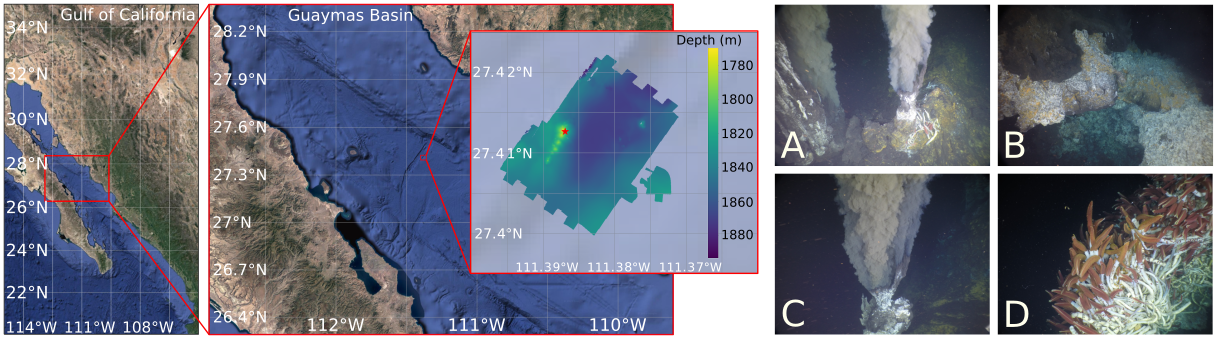
\includegraphics[width=\columnwidth]{figures/site_summary.png}
    \caption{\textbf{Autonomy study site in the Guaymas Basin, Gulf of California.} The inset map is bathymetric data collected by AUV \Sentry during RR2107 and shows the approximately \SI{600}{\meter} long ridge in yellow. The red star marks the chimney used as reference for autonomy studies. Pictures A-D show imagery from the ridge and chimney site. A-C show various forms of plume-producing vents located at the chimney and D shows an example of the macrofauna covering the structures along the ridge.}
    \label{fig:site}
\end{figure}
 

\section{Challenges for Robots and Autonomy in the Deep Ocean}
\label{sec:ops_challenges}
% No GPS, no satellite, only acoustics, very few observatories, etc.
In the Guaymas Basin setting, or any deep ocean research, there are several unique challenges to deploying robotic platforms in contrast to terrestrial applications. Perhaps the most quintessential of these challenges is the conductive nature of water, and its corresponding attenuation of radio frequencies\autocite{qureshi2016rf}. The natural consequence is that ubiquitous terrestrial technologies leveraged by robots and humans alike, such as global position satellites (GPS), imaging satellites, and radio-based wireless communication, are not available for underwater navigation, mapping, or communication. The most common alternative for wireless communication underwater are acoustic waves, which can travel hundreds of kilometers and can be used effectively for ranging (e.g., estimating distance and angle between a source and reflector), but have a significantly reduced data transmission rate. Global positioning of an underwater platform is typically done via acoustic ranging with a ship, the ship having access to GPS. While accurate, the bit-rate and time-of-flight for information transmission is generally not sufficient for constant localization of a vehicle (let alone also requiring a ship to maintain proximity to a platform, and forgo communicating other types of information), and so many state-of-the-art underwater vehicles use a form of ``dead-reckoning'' to estimate their position with inertial sensors. The use of Doppler velocity loggers (DVL), downward facing acoustic sensors that estimate velocity relative to another object, has improved the overall accuracy of dead-reckoning for near seafloor (within \SI{150}{\meter}) navigation. Use of DVL, however, further restricts an AUV to a particular altitude for studies it may conduct under certain localization requirements, either set by the science team or engineering team tasked with keeping the vehicle safe.

Beyond navigation and communication, the challenge of working in water necessarily impacts that type of scientific sensing that can also be accomplished. Light, just like radio, is also severely attenuated in water; sunlight typically only penetrates the ocean to about \SI{200}{\meter}, and up to \SI{1000}{\meter} in the best conditions\footnote{Depths between 200-\SI{1000}{\meter} are aptly part of the ocean's ``Twilight Zone''\autocite{martin2020oceans}}. This means that vision based technologies, which have enjoyed significant development in robotics for e.g., autonomous driving tasks, are entirely restricted to either shallow depths or very near seafloor studies, in which light sources carried by a platform might be used\footnote{Of course, navigating in the water column near no other structure is not necessarily a setting for which vision-based navigation may be useful, nor the data necessarily interesting scientifically.}. Other optical-based sensors, such as Lidar, are similarly not available to be used. Truly, outside of acoustic data products (which can be computationally exhaustive to process in real-time), water-column sensing and mapping in the deep sea relies on collecting point observations and reconstructing fields of interest from these incredibly sparse data.

To address this data sparsity issue, there are several large-scale efforts that contribute to the instrumenting and global understanding of the ocean. Argo, an international network of thousands of small buoyancy-controlled floats which drift in the ocean and take basic \emph{in situ} measurements (e.g., temperature, salinity) of the water column up to \SI{6000}{\meter} in depth is one such example\autocite{roemmich2009argo,jayne2017argo}. With a finer degree of control, small glider networks operated by the e.g., Ocean Observatories Initiative (OOI)\footnote{\url{https://oceanobservatories.org/marine-technologies/gliders/}, \autocite{trowbridge2019ocean}}, offer an opportunity for remote targeting of particular regions or depths to study larger-scale phenomenon. Several highly instrumented ``observatories'', such as Martha's Vineyard Coastal Observatory\autocite{austin2000martha} or the Endurance Array in the Northeast Pacific\autocite{barth2018warm}, also serve an important role for collecting highly temporally resolved data at specific sites. It is certainly the case that there is a lot of ocean data; what has yet to be standardized is how to leverage this data for enabling targeted research studies, particularly with highly capable robotic platforms. Central to this challenge is that despite a wealth of data, the ocean is truly vast; in 10 years of available records from Argo, there are no records of a float in the Guaymas Basin\footnote{As determined via the Euro-Argo data exploration tool, accessed November 20, 2022.}. There are no instrumented arrays in the Gulf of California. And glider or robotics studies conducted there have been part of singular research cruises conducted by disparate research teams, with mixed data discoverability and accessibility. 

\section{Overview of Science Teams and Responsibilities}
%Establish how computer scientists fit on a ship.
Before a robot even touches the water, a massive amount of operational overhead is necessary to support deep sea studies. In general, deep ocean research requires using an oceanographic vessel. The R/V \emph{Revelle} is one of several ships in the University-National Oceanographic Laboratory System (UNOLS) network of research ships available federally supported by the United States\footnote{Private research institutions outside of this network, like the Schmidt Ocean Institute, also provide some global-class ships available for deep sea research.}. The R/V \emph{Revelle}, operated by the Scripps Institution of Oceanography at the University of California, San Diego 

Captain and crew on a research vessel are responsible for the overall safety of the operations, and are key stakeholders in all operations. Marine technicians are crew members that specialize in the scientific instrumentation and infrastructure on a ship, directly working with the science team to assist with deployments and data curation. The science party itself can be a professionally diverse group of trainees and scientists from multiple fields. 

AUV \Sentry is supported by a team of engineers at the National Deep Submergence Facility (NDSF) at Woods Hole Oceanographic Institution (WHOI)\autocite{kaiser2016design}. To deploy \Sentry requires an oceanographic research vessel with suitable winch (to lower \Sentry over the side of the ship, and retrieve it following operations) and workspace to accommodate the on-cruise engineers that includes power and networking capabilities to run the shipboard base station and affiliated sensors.

\section{Data Infrastructure on a Vessel}
Propose live-streaming\dots

\section{Taking Ground Truth Measurements}
Basically impossible, some things more than others.

\subsection{Water Column Standards}
Profiles gathered

\subsection{Hydrothermal Vents}

\subsubsection{Geochemical Measurements}
Jason wand/standard equipment

\subsubsection{Physical Measurements}
Fluid exit velocity, PIV system

\subsection{Crossflow}
Tiltmeters
